\documentclass[conference]{IEEEtran}
\usepackage[utf8]{inputenc}
\usepackage{blindtext, graphicx}
\usepackage{tikz}
% we want ER + above/below + left/right
\usetikzlibrary{er,positioning}
\hyphenation{op-tical net-works semi-conduc-tor}
\usepackage{booktabs} % For formal tables
\usepackage{float}
\usepackage{rotating}

\begin{document}

\title{The usability and buildability of an open source Monitoring Box}

\author{
	\IEEEauthorblockN{Mick Nieman}
	\IEEEauthorblockA{Business IT \& Management\\Amsterdam University\\of Applied Sciences\\
		Wibautstraat 2-4 \\
		1091GM Amsterdam \\
		The Netherlands\\
		Mick.Nieman@hva.nl
		}		
	\and
		\IEEEauthorblockN{Pjotr Scholtze}
		\IEEEauthorblockA{Software Engineering \\Amsterdam University\\of Applied Sciences\\
			Wibautstraat 2-4 \\
			1091GM Amsterdam\\
			The Netherlands\\
			Pjotr.Scholtze@hva.nl
			}			
		\and
			\IEEEauthorblockN{Heeyeon Joung}
			\IEEEauthorblockA{Electrical Engineering\\Seoul National University\\
			of Science and Technology \\
			Seoul Nowon-gu, Gongneung-dong,\\
			Gongneung-ro 232 \\
			South-Korea\\
			Julia.Joung@hva.nl
			}
		}
		
\maketitle	
\thispagestyle{plain}
\pagestyle{plain}

\begin{abstract}
Researchers indicated that there's a Uncertain Geographic Context Problem (UGCoP) \cite{kwan2012uncertain} whilst collecting data. To avoid the Uncertain Geographic Context Problem to occur a data gathering device that is not only capable of collecting sensor data but also GPS-data hands a solution. Now a prototype has been build named 'The Monitoring Box' which is an modular and open-source device which is equipped with a Global Positioning System. Any researcher should be able to re-create the device and also be able to use the device. A device that is not only modular in use but also open-source is not seen before. Our research shows that the average researcher can build 'The Monitoring Box' without expert help or knowledge. The research is done by conducting user-tests and making observations of researchers and students during the build- and use- process of The Monitoring Box. The research shows that there is a relation between the technical level of the researchers or students and the detail-level of the build manual. The current level of detail results in a proven buildability of The Monitoring Box.\\


\end{abstract}

\begin{IEEEkeywords}
Open-source, usability, buildability, environment, environmental logging, data logging, participatory mapping 
\end{IEEEkeywords}

\IEEEpeerreviewmaketitle
\section{Introduction}
There is a need for tools that enable environmental data logging or participatory mapping in order to conduct cetrain research. Currently there are no open source solutions that cover both environmental data capturing and the capturing of the Global Positioning System (GPS)-location. As written in the paper Uncertain Geographic Context Problem \cite{kwan2012uncertain}, uncertain geographic context is still a problem. Researchers that were questioned during the first phases of the research also pointed out that they see a gap between the collected data, from for example data-sprints \footnote{ A group of people, mostly researchers trying to collect as much data as possible to do new findings on a certain topic.}, and the geographical location the data is captured. These gaps result in in-accurate data whilst the accuracy is very important for conducting research as discussed in the paper "The importance of accurate road data for spatial applications in public health: customizing a road network." \cite{frizzelle2009importance}

\par
A lot of similar studies have been done, one of them is "PEIR, the Personal Environmental Impact Report, as a Platform for Participatory Sensing Systems Research"
 \cite{mun2009peir} a paper which also contributes to participatory sensing and environmental mapping using cell phones. In the paper researchers mention that "This calls for new features on both the server side and the handheld device."  \cite{mun2009peir} \\
The Monitoring Box is developed to serve this call. Using the modern day emerged technologies and advanced consumer electronics as, for example FitBit\footnote{ An activity tracker, for more info see https://www.fitbit.com/home}, combined in a hand-held device that can be used for participatory mapping and environmental sensing. At the same time The Monitoring Box is open source and is always available for improvement and adjustment.  

\par
This paper has a selection of questions that serve as a thread. Every subject discussed contributes to answering these questions. The questions asked during this study are: "What factors contribute to creating an open source, multi-research, sensor geolocation aware, data gathering platform"  \cite{monitoringBox2017researchproposal} and "How technical are the students and researchers" along with "What documentation is needed and how detailed should it be?" Also we have taken a closer look at what improves the usability of the product when taking the structure plane of user experience into account. \cite{monitoringBox2017researchproposal} The research proposal of the Monitoring Box also stated the following as a sub-question: "How can the data be made available such that the students \& researchers can use it?" \cite{monitoringBox2017researchproposal} though this question is not as thoroughly studied as the others it has been thought of when answering the main research question.  

\par
This paper is a result of findings made during the development-  and the testing phase of prototype of The Monitoring Box. The paper is written based on the findings made during the research and development and to be learnt from when further developing the monitoring box. It may also be used by others developing similar open sourced data gathering platforms.

\section{Background}
\subsection{Generic articles}
The Mayfly data logger \footnote{ https://envirodiy.org/mayfly/} is an open source data logger for environmental research, they use a customized Arduino. The project is mainly focused on research in a certain environment, for example forests, dunes, swamps and other nature reserves. This project is different from the Monitoring Box because it doesn't use a GPS module for logging its location. The Mayfly data logger is in a fixed position and may only be moved every once in a while. Also it has solar cells with it for recharging its battery and keeps operating for a few days. 
\par
An open source Real Time IOT \footnote{ Internet Of Things} based environmental sensor monitoring sensor \cite{ICRISET2017:An_open_source_Real} Is research done on low cost central sensor data gathering for greenhouses which can allow for optimized crop production. The paper concludes that thinger.io can be used for data gathering, however thinger.io is a paid PAAS\footnote{ Platform As A Service} solution and thus not open source. Besides this, it is real-time which isn't a requirement for our research.
\par
Another project is CKAN\footnote{ https://ckan.org/features/}, which is kind of like a CMS\footnote{ Content Management System} for data. It is an open source solution which allows multiple data sources to be stored on it. You can search multiple datasets with geolocation information such that you can find information about that area, besides that you can also download the datasets and it provides an API \footnote{ Application Programming Interface} for other applications to use. An example of CKAN is\footnote{ https://ckan.org/features/}  which contains almost 1200 datasets about the Netherlands.

\subsection{Data sharing articles}
While the research in this section does not directly applies for the monitoring box, it still is related because it goes into detail of how to handle the data produced by sensor(s) or data that was manually entered.
\par
DBPedia \cite{auer2007dbpedia}  is an open data database based on the datasets available in Wikipedia, but in a better searchable format. This study shows that even if the data is by default easily exchanged it still can be made searchable in a centralized repository. However, it is of course a better idea to make this step unnecessary and allow direct addition to a centralized repository.
\par
RDF (Resource Description Framework) is a format that can be used for exchanging data. \cite{lassila1998resource}  This format uses XML to describe the attributes of the data with their values. This allows for interchangeability and searchability of the data in a centralized manner.
OWL Web Ontology Language Reference \cite{mcguinness2004owl}  is like RDF but it also allows for relationships to other items. This means that one data item can link to another data item and thus describe for example history or something that it is part of.
\par
The open data handbook\footnote{ http://opendatahandbook.org/guide/en/appendices/file-formats/} describes some more formats that can be used for data sharing: JSON, XML, RDF, Spreadsheets, CSVs, text documents, plaintext or HTML, and describes them.
\par
The "Linked sensor data" paper describes an example of publishing sensor data to an open data database\footnote{ http://linkeddata.org/} where a large amount of datasets are available. We can use this to see possible how geolocation aware data can be published and shared.
\par
The paper "Publishing linked sensor data" describes an example with geolocation aware data where its data is published onto the Dbpedia database. \cite{barnaghi2010publishing} 
\subsection{Open Source Articles}
For making the product open source we can look into the Mayfly data logger of EnviroDIY \cite{arscott2017publishing},  which also created an open source sensor data gathering platform and open sourced the hard and software. This research is different from the Monitoring Box because this still requires a certain technical skill level in for example programming, while our research attempts to figure out how to minimize the amount of skill needed.
\par
The "Mapping participatory sensing and community-led environmental monitoring initiatives" \cite{balestrinideliverable} paper describes multiple projects that have participatory mapping of sensor data in cities. This will give a broad view of what already has been created. Thus this paper is not related in a direct manner like a solution, it still describes multiple projects that try to achieve what the Monitoring Box attempts.

\section{Methods}
	In order to conduct the research a prototype is created that can be reproduced multiple times. During the research process further modifications have been applied to the prototype. In order to complete the research we took the following steps:
		\begin{enumerate}
			\item Identify the use cases of the system.
			\item Generalize the use cases to a generic platform design.
			\item Create a prototype.
			\item Research usability concerns.
		\end{enumerate}
		\subsection{Prototype}
			The prototype\footnote{ The software and manuals used for the prototype can be found on GitHub: https://github.com/pjotrscholtze/MonitoringBox} consists of a base station (a Raspberry Pi) and different sensors (using Arduinos). To make sure that the whole setup stayed modular a translation part (the Arduinos) were used. This design ensures that the base station only needs to know one protocol and does not need to know the individual sensors \cite{denti1997designing}. Which allows the base station  to focus on using recording the data, managing data storage and making the sensors dynamically attachable.
			\begin{figure}[ht]
				\centering
				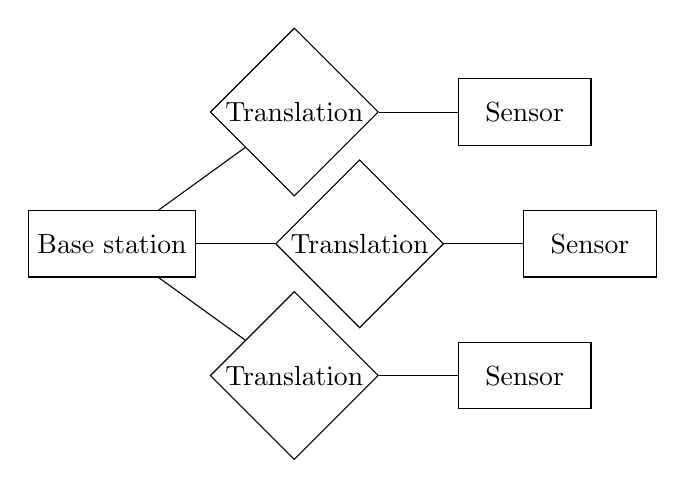
\begin{tikzpicture}[auto,node distance=1cm]
					\node[entity] (node1) {Base station}
									[grow=up,sibling distance=3cm];
					% Now place a relation (ID=rel1)
					\node[relationship] (rel1) [below right = of node1] {Translation};
					\node[relationship] (rel2) [right = of node1] {Translation};
					\node[relationship] (rel3) [above right = of node1] {Translation};
					% Now the 2nd entity (ID=rel2)
					\node[entity] (node2) [right = of rel1]	{Sensor};
					\node[entity] (node3) [right = of rel2]	{Sensor};
					\node[entity] (node4) [right = of rel3]	{Sensor};
					% Draw an edge between rel1 and node1; rel1 and node2
					\path (rel1) edge node {} (node1)
								edge	 node {}	(node2);
					\path (rel2) edge node {} (node1)
								edge	 node {}	(node3);
					\path (rel3) edge node {} (node1)
								edge	 node {}	(node4);
				\end{tikzpicture}
				\caption{Example connection diagram prototype}
			\end{figure}
			\paragraph{Prototype parts}
				\begin{enumerate}
					\item Base station
						\begin{enumerate}
							\item Wi-Fi accesspoint
							\item Web interface
							\item Recording
						\end{enumerate}
					\item Sensors
						\begin{enumerate}
							\item GPS
							\item Temperature and humidity sensor
							\item CO2 sensor (two types)
							\item Heart-rate sensor
							\item Galvanic skin response sensor
							\item Camera (PI-cam)
						\end{enumerate}
				\end{enumerate}
			\paragraph{Prototype features}
				The base station allows all sensors to be plugged and played while turned on, except for the Pi-cam, which is either build in or it is not. Each sensor can be seen on the web interface or via the screen of the base station. The recordings can only be started via the touch screen on the base station. Recordings can be downloaded from the web interface or via an USB stick that can be mounted on the base station. Every sensor is attached to the base station via USB for ease of use and availability of the devices. An USB hub can easily be used to extend the amount of sensors the base station can handle simultaneously. 
		\subsection{Bias}
			Bias is a risk that always occurs when doing research. To avoid bias the researchers have tried not to intervene with the test subjects and only guide them through the process. Only when necessary the researchers would share their point of view with the test subjects. Also during the processing of the outcome of the research and the test the researchers try to have a position as neutral as possible regarding to the topic that is being researched. Another measure taken is the selection of text-subjects. During the testing phase there are a few selected researchers from different backgrounds who applied, this way there is a diversity in the group of selected researchers. The group of students as test-subjects are also selected by their background to have group that is more diverse as only students with the same background. Because of this the bias is kept as minimal as possible with the resources available. It may had been totally absent but this would result in a project-duration longer than the given 10, or 20 when looking at the total project, weeks. We decided to use a fairly diverse group of test subjects, however the size of the group and the diversity could have been bigger by including more faculties.
		\subsection{Research}
			In this section is described how each sub question of our main research question is researched. So as to decide the effective method of research we have considered what we needed to do with the research. We considered what should be focused more between breadth and depth or between quantification and qualification and what would be more efficient in empirical research and desk research in each sub question. Along with these considerations, we have came to the following decision. 

			First, to research 'how technical are the students and researchers', We let students and researchers  use the Monitoring box. Because we wanted to gain various types of students and researchers with different technical levels because the survey panel should be widely spread. With this we can determine what explanation is needed according to the technical level of the student or researcher. So, questions of survey include users' comments so to gain insight in to this. 

			Second, in order to research the question 'What improves the usability of the product when taking the structure plane of user experience into account?', surveys and desk research are conducted and used. And compared afterwards with the shortcomings in usability aspects through existing, similar-functioning platforms and devices. In order to research the Monitoring box in the direction of improving the insufficient aspects of usability.

			Third, in order to research the question 'How can the data be made available in such a way that the students \& researchers can use it?' desk research is used. We studied other similar cases and consider selecting the most appropriate way of data sharing and how researchers use open source and data gathering platforms.
		\paragraph{Interview setup} The interviews were executed in the following order:
			\begin{enumerate}
				\item \textbf{Give the participant general introduction of project to participant.} \\
				Describe the goal, what we are researching and what we they are going to do.
				\item \textbf{Let the participant assemble hardware and upload software.}\\
				Of the MonitoringBox. While he or she is doing the assembly of the prototype we observe participant.
				\item \textbf{Let the participant test built device(s).}\\
				By connecting the sensor to the Raspberry Pi and trying to record.
				\item \textbf{Let the participant use the prototype.}\\
				So that the participant will use all the different features of the software and we observe them.
				\item \textbf{Ask the participant questions from the survey and ask for general feedback.}\\
				Such to get structured information and really find out what the participant thought.
			\end{enumerate}
			The interviews were recorded with a camera and notes were made during this interview. All team members were present during the interviews, one member controlled the camera, one made notes and one did the presentation and guidance.
\section{Results}
<<<<<<< HEAD
Next discussed will be the results, these results refer to the results from our research. As a research we have conducted user tests, interviews and observations. The results of these are shown in the tables and texts below. \\ 

		\begin{figure*}[ht]
=======

	\subsection{Interview participants}
		In order to get an accurate picture of the user group, a sample of users with different backgrounds were chosen. This included students and researchers with different levels of technical skills. The participants of the interviews can be categorized into the following categories:
		\begin{figure}[ht]
			\centering
			\begin{tabular}{ | l | r | l | }
				\hline
				Type			& Amount	& Description \\ \hline \hline
				Researcher		& 2			& Different technical levels* \\ \hline
				Student			& 4			& See figure ... for details \\ \hline \hline
				Total			& 6			& \\ \hline
			\end{tabular}
			\caption{General distribution of participants}
		\end{figure}\\
		The student groups can be sub divided into different sub-categories:
		\begin{figure}[ht]
			\centering
			\begin{tabular}{ | l | r | l | }
				\hline
				Type					& Amount \\ \hline \hline
				Business IT				& 1 \\ \hline
				Game design				& 1 \\ \hline
				Software engineering	& 2 \\ \hline
				Total					& 4 \\ \hline
			\end{tabular}
			\caption{Major of the participating students}
		\end{figure} \\
		This shows users from varying backgrounds participated in the research. However, unfortunately because of time and resources we had limitation in size of this group
		\begin{enumerate}
			\item How technical are the students and researchers?
				\item What documentation is needed and how detailed should it be
				


				\begin{enumerate}
					\item Researcher A\\

						The researcher encountered the following problems during the interview.\\

						First, she does not know how to use a breadboard. To create a Galvanic Skin Response sensor, users have to connect the Arduino Nano, resistor, and several wires. However, these connections are not just one-to-one connections, they require multiple connections. So in order to succeed, users must understand the structure of the breadboard. The manual did not explain the structure of the breadboard, and the researcher had difficulty with it.\\
						Second, she wanted more specified information about cable connections.\\
						The researcher has mentioned that we need the following elements in the document.\\
						First, she suggested that we mention in the manual how to use breadboard and the structure of breadboard. \\
						Second, she suggested that we add more information about Arduino nano and Arduino uno.\\
						Third, she said the manual does not focus in Dutch, but English. \\		
						
					\item Researcher B\\
					Researcher B knows quite a bit of software and has little knowledge of hardware. The researcher encountered the following problems during the interview.\\
					First, he feels there are something unclear about the schematic. 						He pointed out that the schematic pin number is missing. The pin number is too small to specify, so he was uncomfortable with rebuilding.\\
					Second, he was wondering about the difference between the two CO2 sensors. The manual only briefly specifies the name and characteristics of each sensor, but the difference between the two sensors is not specified in detail.\\
					Third, he did not know how to use the breadboard.\\
					The researcher has mentioned that we need the following elements in the document.\\
					First, he suggested that we mention in the manual when to upload and where to see the results. \\
					Second, he suggested links to tutorials about breadboard.\\
					Third, he suggested that we put the technical names in the shopping list\\
					Forth, he suggested that we explain in the manual which part is wrong for each error message.\\
					
					\item Student A\\
					Student A is majoring in Software engineering and has  quite some experience in Arduino. The student A encountered the following problems during the interview.\\
					First, he was confused about the GPS and Arduino nano. He was confused because the GPS and Arduino nano have similar size and similar color.\\
					Second, he had difficulty reading the schematics. The letters in the schematics are too small to read, and it took some time to find out what was written on the next page.\\
					The researcher has mentioned that we need the following elements in the document.\\
					First, he suggested to write the steps in the manual in a bold font.\\
					Second, he suggested adjusting the order of text and schematics. He mentioned that it took a some time to find that there is a text which explain schematics.
					
					\item Student B\\
					Student B is majoring in Game development and has  quite some experience in Arduino. He replied that his technical level is a hobby in the hardware and professional in the software. The student B pointed out the following during the interview.\\
					First, the manual is really easy but it did not state which Arduino sketch is necessary to complete.
					Second, pictures should represent the real life device. Heart rate sensor in the schematics and the real heart rate sensor look different.\\
		\begin{figure*}[!ht]
>>>>>>> 07c018104886005e624d8edc02c4d59e9b560e6d
			\centering
			\begin{tabular}{ | l | l | l | l | l | l | l | l | l | l | }
				\hline
			Participant		& Software issues			& Knowledge gap					& Order issues				& Interface				\\ \hline \hline
			
			
			Researcher A	& COM port selection not	& Does not know what a			& Missing common			& Add icons on buttons,	\\ 
							& repeated					& breadboard, differences		& problem solutions			& link to manual on		\\ 
							& 							& between Arduino types			& 							& device				\\ \hline
							
			Researcher B	& List common error			& Differences between sensors	& how to test sensor,		& Show values during	\\ 
							& messages 					& unkown, does not known 		& describe order to	follow	& recording, stand by	\\
							& 							& how a breadboard works		& for doing	hardware and	& mode for screen, disk	\\
							& 							& know how a bread-				& software					& usage unclear, show	\\
							& 							& board works					& 							& url in WiFi screen	\\	\hline

			Student A		& None						& Difference between GPS and 	& Did not know about the	& It is practical		\\
							&  							& Arduino boards				& description because it 	& 						\\
							&  							& 								& was on the next page		& 						\\ \hline

			Student B		& Unclear what firmware		& Image	should be realistic in	& None						& "It looks fine"		\\ 
							& to upload					& the way that they should be 	& 							& 						\\ 
							&  							& recognizable					& 							& 						\\ \hline
							

			Student C		& It was unclear that you	& Folder structure for firmware& None						& It works, is not too	\\ 
							& need to upload code		& is unclear					& 							& complicated			\\ \hline

			Student D		& It was unclear how to 	& How to connect wires to the	& It was unclear how to 	& Very clear, but could	\\ 
							& upload software			& sensors and Arduino			& code to the Arduino		& have been more pretty	\\ \hline

			Student E		& Did not know what 		& Schematic is hard to follow	& The order of the 			& Add sensor data		\\ 
							& firmware to upload the	& with low knowledge of 		& schematic and description	& preview option so		\\ 
							& folder structure was 		& hardware						& should be reversed		& you know the device	\\ 
							& unclear					& 								& 							& works					\\ \hline
	
			Student F		& Didn't know wen to push	& Didn't know what the which	& Didn't know when to push	& Looks fine, however a	\\ 
							& code						& board was the heart rate 		& code to the Arduino.		& link to the manual	\\
							&  							& board							& 							& would be nice			\\ \hline
			\end{tabular}
			\caption{General distribution of participants}
			\begin{tabular}{ | l | l | l | l | l | l | l | l | l | l | l }
				\hline
					\begin{turn}{-90}Participant\end{turn}			&
					\begin{turn}{-90}Study\end{turn}				&
					\begin{turn}{-90}Age\end{turn}					&
					\begin{turn}{-90}Skill level (1-10)\end{turn}	&
					\begin{turn}{-90}Time taken\end{turn}			&
					\begin{turn}{-90}Humidity\end{turn}			&
					\begin{turn}{-90}CO2\end{turn}					&
					\begin{turn}{-90}GPS\end{turn}					&
					\begin{turn}{-90}GSR\end{turn}					&
					\begin{turn}{-90}Heartrate\end{turn}			
					\\ \hline \hline
			
			
			Researcher A	& N.A.			& 30-35 & 4		& 81	& X	& X	& X	& X	& X	\\ \hline
			Researcher B	& N.A.			& 25-30 & 5 	& 52	& X	& X	& X	& X	& X	\\ \hline
			Student A		& BIM			& 20-25 & 4 	& 25	& 	& X	& X	& X	& 	\\ \hline
			Student B		& GD 			& 25-30 & 8 	& 32	& X	& X	& X	& X	&	\\ \hline
			Student C		& DE			& 20-25 & 5		& 20	& 	& X	& X	&	& X	\\ \hline
			Student D		& SE 			& 25-30	& 9		& 21	& X	& 	& X	& X	&	\\ \hline
			Student E		& BIM		 	& 20-25	& 5 	& 38	& X	&	& X	&	& X	\\ \hline
			Student F		& SE 			& 20-25	& 8		& 39	& X	& X	& X	& X	& X	\\ \hline
			\end{tabular}
			\caption{General distribution of participants}
		\begin{tabular}{ | l | l | }
			\hline
			Abriviation & Study 					\\ \hline \hline
			BIM			& Business It Management	\\ \hline
			GD			& Game Design				\\ \hline
			DE			& Design					\\ \hline
			SE			& Software Engineering		\\ \hline
		
		\end{tabular}
<<<<<<< HEAD
	\subsection{Interviewing of the participants}
		In order to get an accurate picture of the user group, a sample of users with different backgrounds is taken. This includes students and researchers with different levels of technical skills. The participants of the interviews can be categorized into the following categories:
		\begin{figure}[ht]
			\centering
			\begin{tabular}{ | l | r | l | }
				\hline
				Type			& Amount	& Description \\ \hline \hline
				Researcher		& 2			& Different technical levels* \\ \hline
				Student			& 4			& See figure ... for details \\ \hline \hline
				Total			& 6			& \\ \hline
			\end{tabular}
			\caption{General distribution of participants}
		\end{figure}\\
		The student groups can be sub divided into different sub-categories:
		\begin{figure}[ht]
			\centering
			\begin{tabular}{ | l | r | l | }
				\hline
				Type					& Amount \\ \hline \hline
				Business IT				& 1 \\ \hline
				Game design				& 1 \\ \hline
				Software engineering	& 2 \\ \hline
				Total					& 4 \\ \hline
			\end{tabular}
			\caption{Major of the participating students}
		\end{figure} \\
		This shows users from varying backgrounds participated in the research. However, unfortunately because of time and resources we had limitation in size of this group.
		\begin{enumerate}
			\item How technical are the students and researchers?
				\item What documentation is needed and how detailed should it be
				
				\begin{enumerate}
					\item Researcher A\\

						The researcher encountered the following problems during the interview.\\

						First, the researchers does not know how to use a breadboard. To create a Galvanic Skin Response sensor users have to connect the Arduino Nano, a resistor and several wires. However, these connections are not just one-to-one connections, they require multiple connections on a single point. So in order to succeed, users must understand the structure of a breadboard. The manual did not explain the structure of the breadboard because the breadboard is only used during the testing phase. The situation would normally be that the wires are soldered to avoid loose connections. Because of a lack of explanation on breadboards the researcher had difficulty with it.\\
						Second, the researcher wanted more specified information about cable connections.\\
						Afterwards the researcher has mentioned that we need the following elements in the document.\\
						The following elements were suggested by the researcher, starting with the fact that we should mention in the manual how to use a breadboard and how the structure of breadboard functions. \\
						Then she suggested that we add more information about the Arduino nano and Arduino uno.\\
						Finishing with the remark that the manual doesn't focus on Dutch users but is fully written in English.\\		
						
					\item Researcher B\\
					Researcher B knows quite a bit of software and has little knowledge of hardware, as researcher B has technical level 5. The researcher encountered the following problems during the interview.\\
					First, he feels there are some things unclear about the schematics. He pointed out that the schematics' pin number is missing or very unclear. The pin number is too small to specify, so he had to count the amount of pins in order to rebuild.\\
					Second, he was wondering about the difference between the two CO2 sensors. The manual only briefly specifies the name and characteristics of each sensor, but the difference between the two sensors is not specified in detail.\\
					Third, the researcher did not know how to use the breadboard.\\
					The researcher has mentioned that we need the following elements in the document.\\
					First, he suggested that we mention in the manual when to upload and where to see the results. \\
					Second, he suggested links to tutorials about the breadboard.\\
					Third, he suggested that we put the technical names in the shopping list in order to ease the buying of hardware.\\
					Fourth, he suggested that we explain in the manual what the error messages mean and how to solve them instead of only mentioning that there's a possibility of having error messages.\\
					
					\item Student A\\
					Student A is majoring in Software engineering and has  quite some experience in Arduino. Student A encountered the following problems during the interview.\\
					First, he was confused about the GPS and Arduino nano because the GPS and Arduino nano have similar sizes and also have a similar color. Though after taking a closer look at both items the student figured out which item was the GPS and which item was the Arduino.\\
					Second, he had difficulty reading the schematics. The letters in the schematics are too small to read, and it took some time to find out what was written on the next page. This is because the student was mainly focused on the provided schematic and did not mention the explanation of the schematic on the other page.\\
					The researcher has mentioned that we need the following elements in the document.\\
					First, he suggested to write the steps in the manual in a bold font to draw attention to the different steps.\\
					Second, he suggested adjusting the order of text and schematics. He mentioned that it took a some time to find that there is a text which explains the provided schematics.
					
					\item Student B\\
					Student B is majoring in Game development and has  quite some experience in Arduino. He replied that his technical level is higher as average because he practices as a hobby with hardware and is a professional in using software. Student B pointed out the following during the interview.\\
					First, the manual is really easy but it did not state which Arduino sketch is necessary to complete.
					Second, pictures should represent the real life device. Heart rate sensor in the schematics and the real heart rate sensor look different.\\
=======
	\end{figure*}
>>>>>>> 07c018104886005e624d8edc02c4d59e9b560e6d
					
					\item Student C\\
					Student C is majoring in Software engineering and has  quite some experience in Arduino. The student C pointed out the following during the interview.\\
					First, the Galvanic Skin Response schematic is not clear. The Galvanic Skin Response chapter is not in depth enough along with the explanation of how to connect everything. This is because the Galvanic skin response sensor doesn't have a physical sensor but uses two normal wires instead to measure conductance of the skin.\\
					Second, the student asks how the sensor can be tested because the student is not certain if the sensors that were just made are working.\\
					Third, he suggested that the manual explained more information about different cables using a USB connection because the student could not tell the difference.\\

					\item Student D\\
					Student D is majoring in Business IT. He has understanding of user software like programs on Windows and can read code but not write it. Student D pointed out the following during the interview.\\
					First, it is unclear how the wires are connected for the sensor the student wants to create.\\
					Second, the chapter order is not right. The student recommended to put the 'pushing code' chapter the chapters that explain about the assembly of the sensors.\\
					Third, the manual needs more explanation about both the breadboard and the possibility of soldering the connections.\\
					Fourth, the student suggested that the manual shows how the Arduino and computer are connected while pushing code to the Arduino.\\
					He said the Manual is clear but it is not detailed enough. It is unclear where a button is placed on the Arduino Integrated Development Environment and when he has to upload software. Also the student suggested that the manual describes some error messages and add 3D photographs. Because the student thought students with similar levels could have some trouble. 
					
					\item Student E\\
					Student E is majoring in Software engineering and has quite some software skills and has average hardware skills.\\
					The student pointed out the following during the interview.\\
					First, the GSR sensor is tough to follow when not having a lot of hardware experience.\\
					Second, while recording it would have been nice to see the sensor data that is being captured at that very moment, this way you now if the recording is working.\\
					Third, the order of the schematics and descriptions should be reversed in order to make it a better chronological document.
					
					\item Student F\\
					Student F is majoring in Business IT \& Management and is averagely technical-skilled. He has been working with an Arduino before and has read multiple programs in C++ but not actually programmed in C++ by himself.\\
					During the test-phase the student ran into some problems, as listed following.\\
					The first issue he had was with the 'pushing code' chapter which is explained before actually having to push code to the Arduino.\\ 
					This was inconvenient for the user and he suggested that the manual should be written in the same chronological order as the building-steps.\\
					Another remark he made during the building of the heart rate sensor was that it does not look similar to the heart-rate sensor he was holding. \\
When thinking out loud he thought that he doubted if it would have the same functionality then.\\
The student did not have problems with the breadboard.\\
He told that he had seen others use breadboards a lot of times before and he only needed a reminder of what way the wiring would be connected using a breadboard.
				\end{enumerate}
				\newpage

			\item What improves the usability of the product when taking the structure plane of user experience into account?

				The structure plane of user experience and interaction design states that users must communicate correctly with the monitoring box and the monitoring box must deliver the information that the user wants immediately and accurately. In this respect, the Monitoring box has a touch screen and has four menus in this screen so that when the user has the information they want, the user can instantly check the menu. The home screen shows what percentage of the storage capacity is in use and if users select 'Sensor' menu from the Monitoring Box, users can see the currently connected sensors. And if users select 'Wi-Fi' menu from Monitoring Box, users can confirm the Wi-Fi name and password.\\
				In information architecture in the structure plane of user experience, it should facilitate intuitive access to data. So wireless communication is used known as Wi-Fi so that the information can be checked and if the device is connected to the internet. And with a single push of a button on the Web site, users are able to download the data of the sensors the user had recorded at a glance. In addition, the monitoring box screen design allows intuitive use of the menu.
\\

			\item How can the data be made available such that the students \& researchers can use it?
				\begin{enumerate}
					\item In the Monitoring Box
				\begin{enumerate}
			\item Screen
				\begin{enumerate}
					\item Main menu

						In the main menu, there is one bar and four menus. The bar tells users how much storage they have used. This percentage allows the user to see how much memory is left on the SD-card and to control usage. Each menu button has a label to explain its purpose or function.\\
					\item Record

						Users can start recording by pushing this menu. In addition, they can see which sensors are recording while recording.\\
					\item Sensor

						In the Sensor menu, users can see a list of currently connected sensors. It is good to check before recording so that users know the sensors are properly connected.\\
					\item Wi-Fi

						Wi-Fi name and password can be found in this menu. Users do not need to remember or write down the Monitoring Box its Wi-Fi name and password.\\
				\end{enumerate}
			\end{enumerate}
		\item On the Website
			\begin{enumerate}
				\item Wireless connecting to Web page

					The data that users have recorded can be downloaded at once. The wireless data transmitter is used in order to view the data, even if users do not have a certain cable, users can see data only if the user has a Wi-Fi enabled devices such as a laptop, a computer or a smart phone. \\
					A few simple steps are required for users to connect their Monitoring Box to the Web page. First, turn on a Wi-Fi enabled devices and connect the Monitoring box to the Wi-Fi. The Monitoring box is equipped with a Wi-Fi function and the Wi-Fi name and password can be found in the menu on the monitoring box its screen. Then, after you completed the first step, users can go to the monitoring box its website by typing 'monitoring.box:5000' in as a website address.\\

				\item Download the recorded information

					After users access the website, they can see and download the data which they have recorded. The downloadable format is CSV(Comma Separated Value). Because it is truncated in the form of a comma, it can be read not only as a text file but also as an Excel file. When users open CSV file in Excel, the user can view and store the sorted data in sequence.\\

				\item Graph

					Users can view a list of currently connected sensors in real time on the web page and a graph of their sensor values. Users can easily access data and see the data at a glance.\\
			\end{enumerate}
		\end{enumerate}
 	\end{enumerate}
\section{Conclusion}
	This has no content yet or is a work in progress and thus not yet shown.

\section{Discussion}
	Looking at the main research question it could be said that there is a variety of factors that contribute to the successful creation of an open source, multi-research, sensor geolocation aware, data gathering platform that can be used by the students and researchers. The usability is different for every device and modification of a device. Slight alternations may result in a total different user experience and the usability aspects. \\
	When creating a device that is similar to the open source, environmental data-logger used for participatory mapping device called The Monitoring Box it is important to know the user group it is being developed for. Depending on the technical level of the user group there needs to be adjustments made to the manual. Is the technical level rated from 7 to 10 the manual does not need the level of detail needed when the technical level is rated below 4. Between 4 and 7 is a gap that may need a high level of detail or be able to make it without.\\
	Another important aspect of having an open source monitoring box is the availability of the used hardware. Every used part of hardware for the Monitoring box can be bought in store as-is. There is no dependency on a supplier or manufacturer linked to 'The Monitoring Box'. Of course it might occur a manufacturer of supplier can't deliver the right piece of hardware though in this case the system is prepared to handle similar pieces of hardware as long as it has the same characteristics as the previous piece of hardware. \\
	The final important discovery is the availability of the written software. As thought of and researched during the development of The Monitoring Box it has been decided that the hosting is something easily done by sites that provide a free platform for hosting open source software.\\	
	As there are not much projects similar to this project the main difference shows that this project has no 'custom made' items. Everything can be bought as separate parts from different suppliers. Though this requires extra work it provides a higher certainty of availability of these parts. \\
	It could be said that this report and the results of the research only apply to the Monitoring Box. This is partially true, though any researcher or developer well informed about the topic they are going to research on or work for can determine what results may apply to their product and what may not.

\section{Future works}
	In order for this study to be in more depth, suggested is to perform further research to the future works explained as follows. \\
	The first future work suggestion is about the master students that were unavailable for this research. The resources needed to recruit them were not available nor were the students themselves. Interviews with master's degree students will improve the results of the study. Because this is in elaboration of the study performed by this research. Having a bigger scope results in more accurate results.\\
	Second, the people with different backgrounds and different knowledge levels could participate to a group interview. Interviewing for usability and buildability of the Monitoring Box with more people from different majors can improve the results of the research. Because it enlarges the scope of the selected user group and thus results in more accurate results.\\
	Third, Further research might have been conducted on  the following topic. This is something that should been done as further research: "How can the data be made available such that the students \& researchers can use it?" Because of limited time and currently not having the need of researching this. Though using this topic will help you validate and improve the usability of the Monitoring Box or similar projects.\\
	Finishing with the need of improvement in design. The  Monitoring Box is equipped with various sensors as well as Global Positioning System. Since users have to carry the device around, a design that allows users to carry the device around in a more convenient way the design  of the Monitoring Box needs to be further researched.\\
	
\section{Acknowledgements}
We would like to pay our regards to our fellow researchers of the Minor Research in Emerging Technologies. \\
Also we would like to show our gratitude to our teachers Joey van der Bie, Nazli Cila, Jurriaan Mulder and Bas Pijls. For teaching us the necessary skills in order to accomplish the project and this paper. \\
 The following thank you is for the researchers of the Citizen Data Lab and the Makerslab. \\ 
Our special thanks are for our teacher, coach and client Wouter Meys and our client Loes Bogers. Without you we would not have had fun doing our project. 

\bibliographystyle{plain}
\bibliography{Research_Report_Monitoring_Box_IEEE_Style}

\end{document}